\documentclass[aspectratio=169,11pt]{beamer}
\usepackage[T1]{fontenc}
\usepackage{lmodern,amsmath,amssymb,mathtools,bm,booktabs,array,graphicx,tikz}
\usetikzlibrary{arrows.meta,positioning,calc,decorations.pathreplacing,patterns}
\definecolor{ink}{HTML}{17344D}\definecolor{accent}{HTML}{087E8B}\definecolor{pale}{HTML}{EDF5F5}\definecolor{gold}{HTML}{AD6B19}
\providecommand{\dd}{\,\mathrm{d}}\providecommand{\R}{\mathbb{R}}
\providecommand{\E}{\mathbb{E}}\providecommand{\Var}{\operatorname{Var}}
\providecommand{\Cov}{\operatorname{Cov}}\providecommand{\diag}{\operatorname{diag}}
\providecommand{\norm}[1]{\left\lVert#1\right\rVert}
\providecommand{\abs}[1]{\left|#1\right|}
\usefonttheme{professionalfonts}
\setbeamercolor{normal text}{fg=black,bg=white}
\setbeamercolor{frametitle}{fg=ink,bg=white}
\setbeamercolor{title}{fg=ink}\setbeamercolor{structure}{fg=accent}
\setbeamercolor{block title}{fg=ink,bg=pale}\setbeamercolor{block body}{fg=black,bg=pale!40}
\setbeamercolor{alerted text}{fg=accent}
\setbeamerfont{frametitle}{size=\Large,series=\bfseries}
\setbeamerfont{title}{size=\LARGE,series=\bfseries}
\setbeamertemplate{navigation symbols}{}
\setbeamersize{text margin left=.7cm,text margin right=.7cm}
\setbeamertemplate{frametitle}{\vspace{.18cm}\insertframetitle\par\vspace{.1cm}{\color{accent}\hrule height .6pt}\vspace{.12cm}}
\newcommand{\notestarget}{notes.pdf}\newcommand{\noteslabel}{Notes}
\setbeamertemplate{footline}{\hspace{.7cm}\color{ink}\scriptsize Mathematical Cardiology\quad\href{\notestarget}{\noteslabel}\hfill\insertframenumber\,/\,\inserttotalframenumber\hspace{.7cm}\vspace{.18cm}}
\setbeamercovered{invisible}
\hypersetup{pdfauthor={Zan Ahmad},pdftitle={Feedback, stability, and hydrostatic pressure},pdfpagemode=UseNone}
\begin{document}
\begin{frame}[plain]\vfill
{\small\color{accent} Mathematical Cardiology \quad Lecture 6}\par\medskip
{\raggedright\hyphenpenalty=10000\exhyphenpenalty=10000\LARGE\bfseries\color{ink} Feedback, stability, and hydrostatic pressure}\par\bigskip
Zan Ahmad\par\smallskip
{\small Fall 2023}\par\vfill\end{frame}
\renewcommand{\notestarget}{notes.pdf\#note-closing-the-pressure-loop}
\begin{frame}[t,fragile,label=slide-pressure-as-a-function-of-rate]{Pressure as a function of rate}
With fixed stroke volume,
\[Q=HV_s/1000.\]
\pause{}
With one downstream resistance,
\[P=P_v+RQ=P_v+aH,\qquad a=RV_s/1000.\]
$H$ is in beats/min and $Q$ is in L/min.
\end{frame}
\renewcommand{\notestarget}{notes.pdf\#note-closing-the-pressure-loop}
\begin{frame}[t,fragile,label=slide-the-initial-pressure]{The initial pressure}
\[V_s=100,\quad P_v=5,\quad R=15,\quad H=60.\]
\pause{}
\[Q=6\,\mathrm{L/min},\qquad P=5+15(6)=95\,\mathrm{mmHg}.\]
The equation describes a mean pressure; it contains no pulse or storage state.
\end{frame}
\renewcommand{\notestarget}{notes.pdf\#note-closing-the-pressure-loop}
\begin{frame}[t,fragile,label=slide-a-resistance-disturbance]{A resistance disturbance}
Hold $H=60$ and let $R$ fall from $15$ to $10$.
\[P=5+10(6)=65\,\mathrm{mmHg}.\]
\pause{}
For a $95\,\mathrm{mmHg}$ target,
\[P_*-P=30\,\mathrm{mmHg}.\]
This error is the input to the next correction.
\end{frame}
\renewcommand{\notestarget}{notes.pdf\#note-a-discrete-correction-rule}
\begin{frame}[label=slide-a-measured-error-changes-the-next-rate-figure]{A measured error changes the next rate}
\centering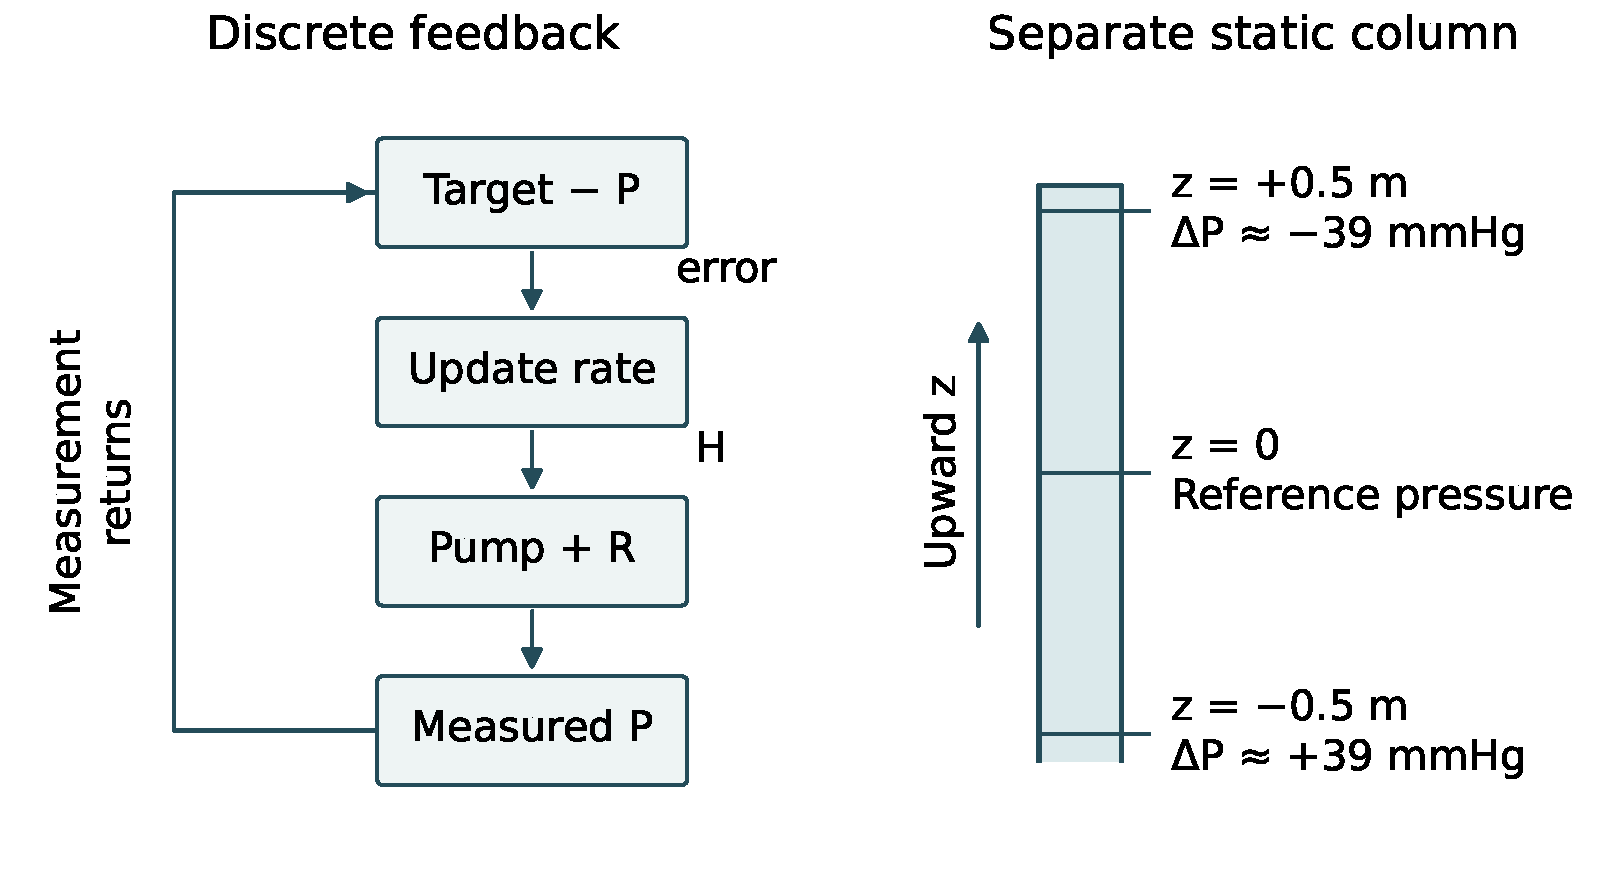
\includegraphics[width=.98\linewidth,height=.69\textheight,keepaspectratio]{feedback-and-height.pdf}\end{frame}
\renewcommand{\notestarget}{notes.pdf\#note-a-discrete-correction-rule}
\begin{frame}[t,fragile,label=slide-a-measured-error-changes-the-next-rate]{A measured error changes the next rate}
\[H_{n+1}=H_n+k(P_*-P_n),\qquad P_n=P_v+aH_n.\]
\pause{}
Use $k=0.5$ once every ten seconds.
\[H_1=60+0.5(95-65)=75\,\mathrm{beats/min}.\]
Then $P_1=5+75=80\,\mathrm{mmHg}$.
\end{frame}
\renewcommand{\notestarget}{notes.pdf\#note-a-discrete-correction-rule}
\begin{frame}[t,fragile,label=slide-continue-the-recurrence]{Continue the recurrence}
At $R=10$, $P_n=5+H_n$.
\[
\begin{array}{c|rrrr}
n&0&1&2&3\\\hline
H_n&60&75&82.5&86.25\\
P_n&65&80&87.5&91.25
\end{array}
\]
\pause{}
Each pressure error is half the preceding error. Why?
\end{frame}
\renewcommand{\notestarget}{notes.pdf\#note-equilibrium-and-the-error-multiplier}
\begin{frame}[t,fragile,label=slide-find-the-equilibrium-first]{Find the equilibrium first}
At equilibrium, $H_{n+1}=H_n=H_*$.
\[0=k(P_*-P_v-aH_*).\]
\pause{}
For $k\ne0$ and $a>0$,
\[H_*=(P_*-P_v)/a.\]
Here $H_*=90\,\mathrm{beats/min}$.
\end{frame}
\renewcommand{\notestarget}{notes.pdf\#note-equilibrium-and-the-error-multiplier}
\begin{frame}[t,fragile,label=slide-subtract-the-equilibrium]{Subtract the equilibrium}
Put $e_n=H_n-H_*$. Since $P_*-P_v=aH_*$,
\[e_{n+1}=e_n-kae_n.\]
\pause{}
Thus
\[\boxed{e_{n+1}=(1-ka)e_n},\qquad e_n=(1-ka)^n e_0.\]
\end{frame}
\renewcommand{\notestarget}{notes.pdf\#note-equilibrium-and-the-error-multiplier}
\begin{frame}[t,fragile,label=slide-read-stability-from-one-multiplier]{Read stability from one multiplier}
Let $r=1-ka$.
\[e_n=r^n e_0.\]
\pause{}
\begin{tabular}{ll}
$0<ka<1$&same-sign shrinking errors\\
$ka=1$&one-step correction\\
$1<ka<2$&alternating shrinking errors\\
$ka=2$&persistent alternation
\end{tabular}
\pause{}
Convergence requires $|r|<1$.
\end{frame}
\renewcommand{\notestarget}{notes.pdf\#note-equilibrium-and-the-error-multiplier}
\begin{frame}[label=slide-the-actual-pressure-sequence-figure]{The actual pressure sequence}
\centering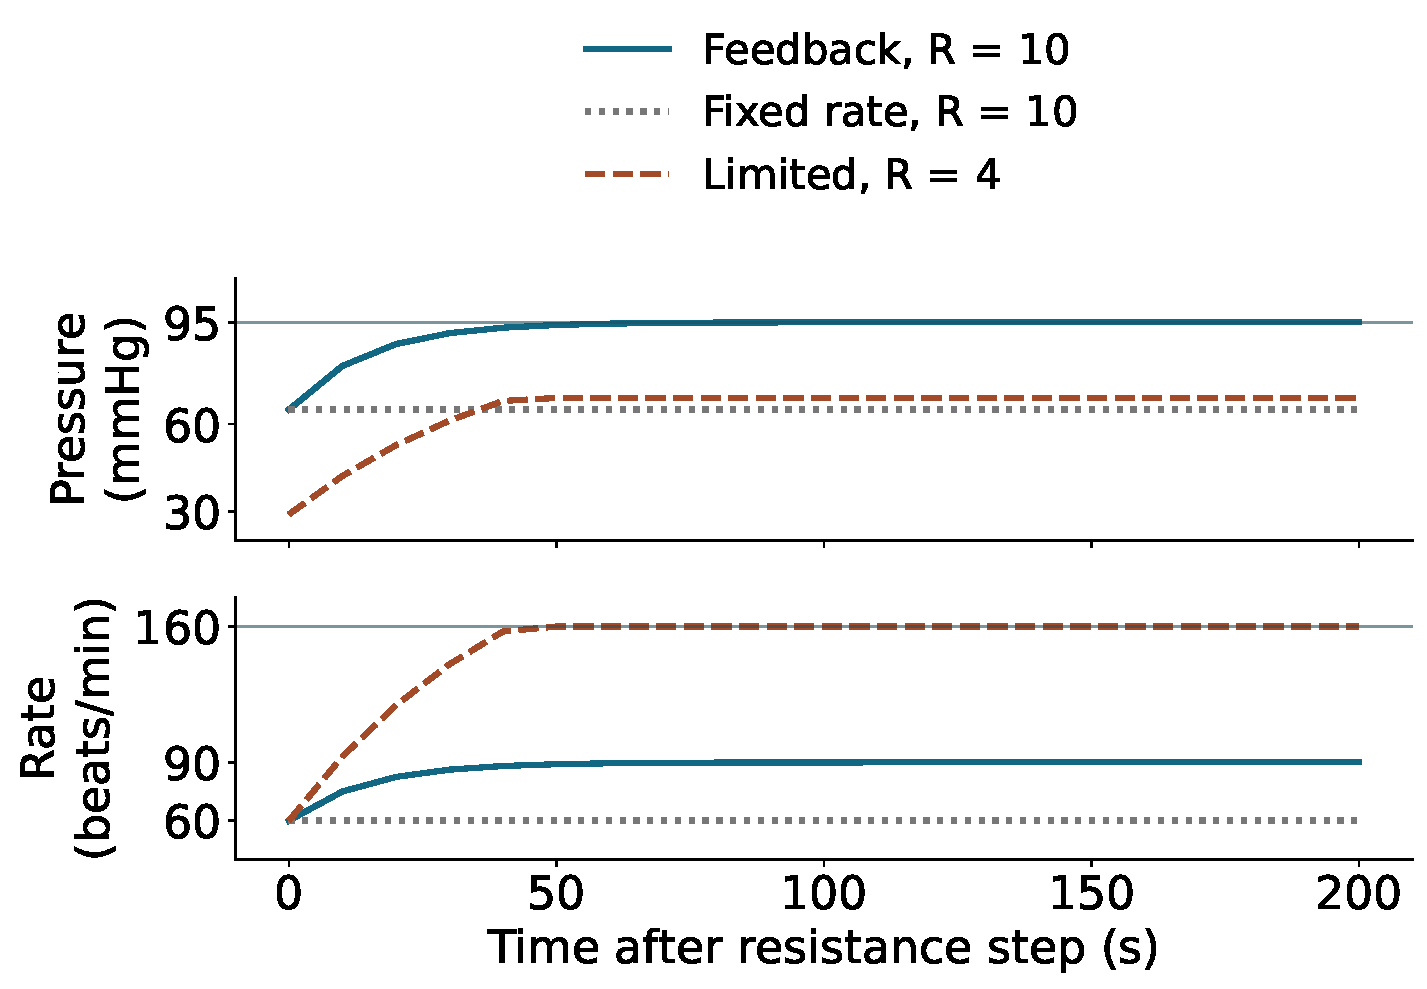
\includegraphics[width=.98\linewidth,height=.69\textheight,keepaspectratio]{feedback-response.pdf}\end{frame}
\renewcommand{\notestarget}{notes.pdf\#note-equilibrium-and-the-error-multiplier}
\begin{frame}[t,fragile,label=slide-the-actual-pressure-sequence]{The actual pressure sequence}
For $ka=0.5$, $H_0-H_*=-30$.
\[H_n=90-30(1/2)^n,\qquad P_n=95-30(1/2)^n.\]
\pause{}
Each factor of $1/2$ takes ten seconds in this experiment.
\end{frame}
\renewcommand{\notestarget}{notes.pdf\#note-an-attainable-target-and-a-saturated-controller}
\begin{frame}[t,fragile,label=slide-the-rate-cannot-increase-without-bound]{The rate cannot increase without bound}
The implementation clips the proposed rate to $[40,160]$.
\pause{}
At $R=4$,
\[H_*=(95-5)/0.4=225>160.\]
\pause{}
At the upper bound,
\[P=5+0.4(160)=69\,\mathrm{mmHg}.\]
\end{frame}
\renewcommand{\notestarget}{notes.pdf\#note-an-attainable-target-and-a-saturated-controller}
\begin{frame}[t,fragile,label=slide-why-more-gain-does-not-solve-this-case]{Why more gain does not solve this case}
The largest available flow is
\[Q_{\max}=160(100)/1000=16\,\mathrm{L/min}.\]
\pause{}
The largest available pressure is $69\,\mathrm{mmHg}$.
The residual error is $95-69=26\,\mathrm{mmHg}$.

Changing $k$ cannot change this bound.
\end{frame}
\renewcommand{\notestarget}{notes.pdf\#note-closing-the-pressure-loop}
\begin{frame}[t,fragile,label=slide-physiological-feedback-mechanisms]{Physiological feedback mechanisms}
The recurrence has one sensor, one scalar error and one actuator.
\pause{}
A baroreflex can alter vascular and cardiac behavior, including mechanisms absent from $P=P_v+aH$.

Delays and additional states can change the multiplier calculation.
\end{frame}
\renewcommand{\notestarget}{notes.pdf\#note-a-hydrostatic-pressure-difference}
\begin{frame}[t,fragile,label=slide-the-weight-of-a-static-column]{The weight of a static column}
A column of depth $d$ and area $A$ has weight $\rho Adg$.
\[(P_{\mathrm{bottom}}-P_{\mathrm{top}})A=\rho Adg.\]
\pause{}
\[\boxed{P_{\mathrm{bottom}}-P_{\mathrm{top}}=\rho gd}.\]
\end{frame}
\renewcommand{\notestarget}{notes.pdf\#note-a-hydrostatic-pressure-difference}
\begin{frame}[t,fragile,label=slide-half-a-meter-below-the-reference]{Half a meter below the reference}
\[\Delta P=1060(9.81)(0.5)=5199.3\,\mathrm{Pa}.\]
\pause{}
\[\Delta P=5199.3/133.322\simeq39.0\,\mathrm{mmHg}.\]
If $z$ increases upward, $\Delta P=-\rho g\Delta z$.
\end{frame}
\renewcommand{\notestarget}{notes.pdf\#note-a-hydrostatic-pressure-difference}
\begin{frame}[t,fragile,label=slide-a-column-is-not-an-orthostatic-model]{A column is not an orthostatic model}
Around a loop returning to its starting height,
\[\sum \Delta z=0\quad\Longrightarrow\quad\sum(-\rho g\Delta z)=0.\]
\pause{}
The displayed controller contains no height input, venous pooling, or posture-dependent stroke volume.
\end{frame}
\end{document}
